\documentclass[11pt]{article}

\usepackage[utf8]{inputenc}
\usepackage[T1]{fontenc}
\usepackage{lmodern}
\usepackage{microtype}
\usepackage[margin=2.5cm]{geometry}
\usepackage{amsmath,amssymb,amsthm,mathtools}
\usepackage{graphicx}
\usepackage{booktabs}
\usepackage{array}
\usepackage{float}
\usepackage[section]{placeins}
\usepackage[dvipsnames]{xcolor}
\usepackage[numbers,sort&compress]{natbib}
\usepackage[colorlinks=true,linkcolor=blue!60!black,citecolor=green!50!black,urlcolor=blue!70!black]{hyperref}
\usepackage{cleveref}

\newcommand{\R}{\mathbb{R}}
\newcommand{\BW}{\mathrm{BW}}
\theoremstyle{remark}
\newtheorem{remark}{Remark}

\title{Decomposed Velocity Fields During Grokking}
\author{Tom\'as Flood\\School of Mathematics and Statistics\\The University of Melbourne}
\date{}

\begin{document}

\maketitle

\begin{abstract}
Grokking refers to the phenomenon of neural networks hitting near-perfect training accuracy early and then taking orders of magnitude more steps to generalise on a held-out dataset \citep{power2022grokking}. The primary contribution is a pointwise velocity-field Hodge decomposition across three grokking runs. The spatial analysis showed that, in the baseline seed, the probe velocity evolves from a coexact-dominated (curl-like, $\sim$49\%) regime during memorisation to an exact-dominated (directed, $\sim$69\%) post-grokking regime, with the exact component rising during the transition window (epochs 1{,}500 to 4{,}000). Across three seeds the coexact fraction in this window is 0.48--0.56, peaking at the start of the transition in two of them. Effective dimensionality and resolvent BW distance provide global corroborating diagnostics. Further, a stronger mechanistic claim would also require the Hodge decomposition to survive parameter and probe sweeps, which we were not able to complete due to resource constraints.
\end{abstract}

\section{Introduction}

Grokking refers to the phenomenon of neural networks hitting near-perfect training accuracy early and then taking orders of magnitude more steps to generalise on a held-out dataset \citep{power2022grokking}. The delay arises not from a lack of capacity but from the time the network takes to find a representation that generalises from data it can already fit.

The network first memorises the training set as a lookup table, then gradually finds a compact algorithmic solution. For modular addition $(a + b) \bmod P$ with $P$ prime, \citet{nanda2023progress} used mechanistic interpretability to show that the generalising solution is a Fourier representation. The solution learned embeds each residue class $a \in \mathbb{Z}/P\mathbb{Z}$ as a point on a circle in a 2D subspace, with the angular position of $a$ being $2\pi k a / P$ for some frequency~$k$. Addition then follows from the trigonometric identity
\begin{equation}
\cos\!\bigl(\tfrac{2\pi k (a+b)}{P}\bigr) = \cos\!\bigl(\tfrac{2\pi k a}{P}\bigr)\cos\!\bigl(\tfrac{2\pi k b}{P}\bigr) - \sin\!\bigl(\tfrac{2\pi k a}{P}\bigr)\sin\!\bigl(\tfrac{2\pi k b}{P}\bigr).
\label{eq:clock-identity}
\end{equation}
This clock algorithm needs only a small number of Fourier frequencies. It places the $P$ residue classes on a low-dimensional manifold with the topology of a circle for one frequency or a torus for several.

The primary contribution is a pointwise velocity-field Hodge decomposition across three grokking runs. The transition is clearly visible in the representation and in the global corroborating diagnostics. Supplementary geometric diagnostics and an audit of the evidential status of these claims appear in the appendix.

In this paper we study the grokking transition through a primary spatial analysis and complementary global diagnostics. Both are built on a shared representation space made from activation checkpoints.

\begin{enumerate}
    \item Primary spatial analysis. The probe displacement field $v_i(t) = x_i(t + \Delta t) - x_i(t)$ between consecutive checkpoints is a vector field on the point cloud at time~$t$. We treat it as a degree-1 object and perform Hodge decomposition via DiffusionGeometry, partitioning the velocity into exact (gradient), coexact (curl), and harmonic components.

    \item Global corroborating diagnostics. We track the effective dimension of the centred activation covariance. At each checkpoint we also build the graph Laplacian $L_t$ and derive the regularised inverse, or resolvent covariance, $\Sigma_t = (L_t + \varepsilon I)^{-1}$ on the retained non-trivial spectral subspace, an inversion which emphasises low-frequency structure. We measure the Bures--Wasserstein distance between consecutive Gaussians.
\end{enumerate}

The spatial analysis captures what the representation is \emph{doing}, by tracking how activation vectors move between checkpoints. The global diagnostics capture how the representation and its diffusion geometry evolve.

\section{Experimental Setup}

\subsection{Architecture and Training}

The training setup follows \citet{nanda2023progress} verbatim except for the single-head reduction discussed below; we record the parameters here for completeness.

We use a deliberately simplified single-head variant of the \citet{nanda2023progress} architecture:
\begin{itemize}
    \item Task: modular addition $(a + b) \bmod 113$, with $P = 113$ (prime).
    \item Architecture: 1-layer transformer (TransformerLens~2.17.0), embedding dimension $d_{\mathrm{model}} = 128$, single attention head ($d_{\mathrm{head}} = 128$), MLP hidden dimension 512, no layer normalisation.
    \item Optimiser: AdamW with $\beta = (0.9, 0.98)$, weight decay $1.0$.
    \item Training: 25{,}000 epochs, full-batch.
    \item Data split: 70\% of all $(a, b)$ pairs held out for validation.
    \item Reproducibility: \texttt{torch.manual\_seed(598)} before model creation; no separate model seed. Pinned to TransformerLens~2.17.0. In the runs checked, this setup reproduces across TL versions 2.9.0--2.17.0.
\end{itemize}

We intentionally did not aim for an exact reproduction of the four-head model in \citet{nanda2023progress}. We reduced to a single head because the four-head version gave a noisier representation. In that version the circular correlation of the recovered coordinates falls from $\approx 0.85$ to $\approx 0.44$, which makes the Fourier analysis we run later quite difficult. Indeed, the 1-head variant shows the same memorisation, transition and generalisation pattern that we want to analyse, and we found the Fourier geometry easier to read.

At 51 checkpoints (every 500 epochs plus initialisation) we extract the MLP hidden activations (post-ReLU, $n_{\mathrm{hidden}} = 512$) at the ``$=$'' token position for a fixed probe set of $n = 500$ subsampled input pairs. This gives a sequence of point clouds $X_t \in \R^{500 \times 512}$.

\subsection{Methods}

\paragraph{Spatial side: DG velocity Hodge decomposition.} Given consecutive checkpoints $X_t$ and $X_{t+\Delta t}$, the probe displacement field is
\[
v_i(t) = x_i(t+\Delta t) - x_i(t).
\]
We reduce $X_t$ to 10 dimensions with PCA. We also project $v_i$ through the same basis. We then build a DiffusionGeometry model \citep{jones2025diffusion,jones2026computing} with $k$NN${}=15$ and 50 spectral basis functions on the reduced point cloud. We promote the displacement to a degree-1 form and apply the Hodge decomposition
\[
\omega = \mathrm{d} f + \delta g + h,
\]
where $\mathrm{d} f$ is exact (the gradient of a 0-form), $\delta g$ is coexact (the codifferential of a 2-form), and $h$ is harmonic. The three components are orthogonal on a smooth manifold. On a finite point cloud the numerical cross terms are small but non-zero. The raw magnitude charts are very noisy, so to interpret them we look at the composition rather than the raw magnitudes. We report normalised energy fractions $(\hat{e}_{\mathrm{exact}}, \hat{e}_{\mathrm{coexact}}, \hat{e}_{\mathrm{harmonic}})$ that sum to one by construction, telling us how much of the probes' motion is gradient-like, coexact-like, or left in the residual harmonic component. We read the harmonic term conservatively in this chapter: without an independent persistent homology or Betti number calculation we cannot treat the harmonic energy as direct evidence for a topological cycle.

\paragraph{Operator side: resolvent BW distance.} At each checkpoint we build the symmetric normalised graph Laplacian $L_t$ (adaptive-bandwidth Gaussian kernel, $k$NN${}=15$) on the PCA-reduced probe cloud \citep{coifman2006diffusion} and extract $K = 30$ non-trivial eigenpairs, excluding the constant mode. The resolvent covariance is $\Sigma_t = (L_t + \varepsilon I)^{-1}$ on this retained non-trivial spectrum, with $\varepsilon = 0.01$, which maps small non-trivial Laplacian eigenvalues to large covariance eigenvalues and so emphasises low-frequency structure. We compute the BW distance $d_{\BW}(\Sigma_t, \Sigma_{t+\Delta t})$ between consecutive checkpoints \citep{bhatia2019bures}.

Given two geometric states as Gaussians $\mathcal{N}(0, \Sigma_0)$ and $\mathcal{N}(0, \Sigma_1)$ where $\Sigma_t = f(L_t)$, the Bures--Wasserstein distance \citep{bhatia2019bures} is:
\begin{equation}
d_{\BW}^2(\Sigma_0, \Sigma_1)
= \operatorname{tr}(\Sigma_0) + \operatorname{tr}(\Sigma_1)
- 2\,\operatorname{tr}\!\left[\left(\Sigma_0^{1/2} \Sigma_1 \Sigma_0^{1/2}\right)^{1/2}\right].
\label{eq:bw-distance}
\end{equation}
This equals the Wasserstein-2 distance $W_2(\mathcal{N}(0,\Sigma_0), \mathcal{N}(0,\Sigma_1))$. Each Gaussian encodes the diffusion geometry of its manifold, and the BW distance is the cost of morphing one geometry into the other.

\subsection{Scope and Limitations}

The quantitative analysis within this paper is a three-seed case study, and any other run was used only to check our results; those runs sit outside the main pipeline. We also ran a probe robustness check on the global corroborating diagnostics: effective dimensionality and resolvent BW distance. Across four random 400-example subsets, the dimensional collapse and the BW spiking at the transition point survive.

The Hodge decomposition operates on the same static set of 500 probe examples. Because resampling probes could affect consistency, uncertainty remains around how stable these results are. A more thorough robustness check using repeated probing was tried, along with varying key settings in the Hodge process of the pipeline. These attempts ran into hard limits on memory capacity before finishing. Incomplete due to resource constraints, those expanded tests appear here without full data coverage.

The results of this paper should be read as findings from three carefully analysed training runs. Changing the configurations slightly can alter the figures even when trends look stable. Our conclusions therefore remain bound to the setup used and nothing broader.

Lastly, the Hodge fractions shift with changes to the PCA dimension, along with adjustments to both neighbourhood range and the spectral cutoff used. All results below come from one configuration and three seeds rather than a sweep of a larger seed bank.

\section{Results}

\subsection{Training Dynamics}

A few hundred rounds into training the model hits perfect training accuracy. Yet when tested on unseen data, performance barely beats random guessing until epoch 1{,}500. From that point forward improvement accelerates past the tipping point, reaching 94.3\% validation accuracy by epoch 3{,}000 and 100\% by epoch 4{,}000.

Later analyses tie back to this timeline as their foundation. Training divides into three segments: \emph{memorisation} occurs between epochs 0 and 1{,}500. The shift known as \emph{grokking} unfolds from epoch 1{,}500 onward, lasting until around epoch 4{,}000. Beyond that point performance settles, which marks the \emph{post-grokking} period. Large shifts in validation accuracy, along with changes in how representations are structured, define what we call a phase transition; we use ``phase transition'' descriptively, as an analogy of a thermodynamic phase transition.

We created the following event study to show that the same geometric pattern appears at the transition in all three seeds. To compare the runs in the same chart, we indexed each run by the first checkpoint at which it reached a validation accuracy of 0.5. The result in \Cref{fig:grokking-event-study} shows that the dimensional collapse, validation accuracy transition, BW distances and coexact-led Hodge decomposition are all present at the generalisation transition across the three seeds.

\begin{figure}[htbp]
\centering
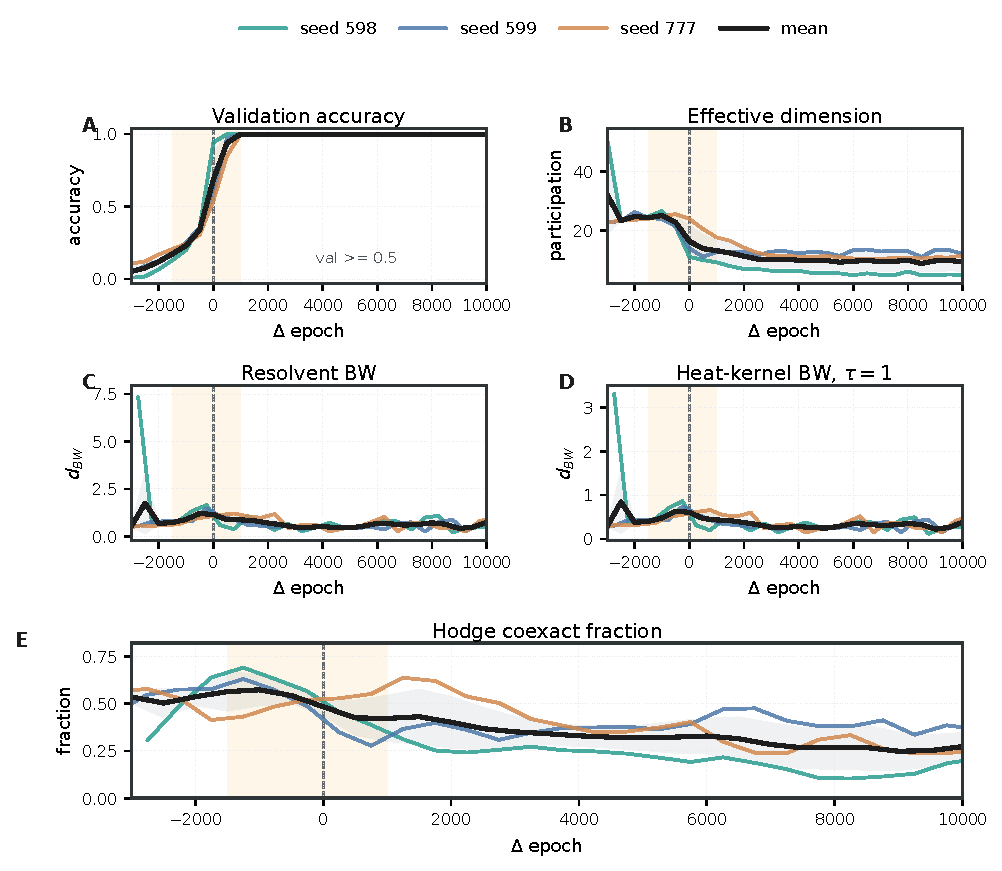
\includegraphics[width=\textwidth]{figures/fig_grokking_event_study.pdf}
\caption{Three-seed event study aligned by the first checkpoint where validation accuracy reaches 0.5. Panel A shows validation accuracy. Panel B shows effective dimension. Panel C shows consecutive resolvent BW distance. Panel D shows consecutive heat-kernel BW distance at $\tau=1$. Panel E shows the Hodge coexact fraction.}
\label{fig:grokking-event-study}
\end{figure}

\subsection{Spatial Side: Velocity Hodge Decomposition}

\Cref{fig:dg-velocity-hodge} shows the DG smooth Hodge decomposition of the probe displacement field across all 50 consecutive checkpoint pairs. The character of the velocity changes at the grokking transition:

\begin{enumerate}
    \item Memorisation phase (epochs 0--1{,}500): the velocity is coexact-dominated on average (mean $\sim$49\% coexact, $\sim$32\% exact, $\sim$19\% harmonic). Step 1{,}000$\to$1{,}500 shows the strongest coexact fraction ($\sim$72\%). This indicates curl-dominated rearrangement of the point cloud during memorisation. The initial step 0$\to$500 still behaves differently, with elevated harmonic energy ($\sim$36\%); this likely reflects large-scale compression from random initialisation and residual global structure in the harmonic component rather than direct topological evidence.

    \item Grokking transition (epochs 1{,}500--4{,}000): the exact component rises within the window as the Fourier structure emerges, but the phase remains coexact-leading on average ($\sim$33\% exact, $\sim$54\% coexact, $\sim$13\% harmonic). The transition is therefore a gradual rise of exact motion within a still-curl-dominated regime, with the actual flip happening only post-grokking in the baseline seed. Across three seeds the coexact fraction in this window is 0.48--0.56, peaking at the start of the transition in two of them.

    \item Post-grokking (epochs 4{,}000+): the exact component leads on average (mean $\sim$69\% exact, $\sim$21\% coexact, $\sim$10\% harmonic). The representation continues to undergo directed refinement, while the harmonic term remains a residual global component of the finite DG decomposition rather than direct evidence for a topological cycle. Note that across three seeds the composition varies (post-grokking exact fraction 0.24--0.69).
\end{enumerate}

\begin{figure}[htbp]
\centering
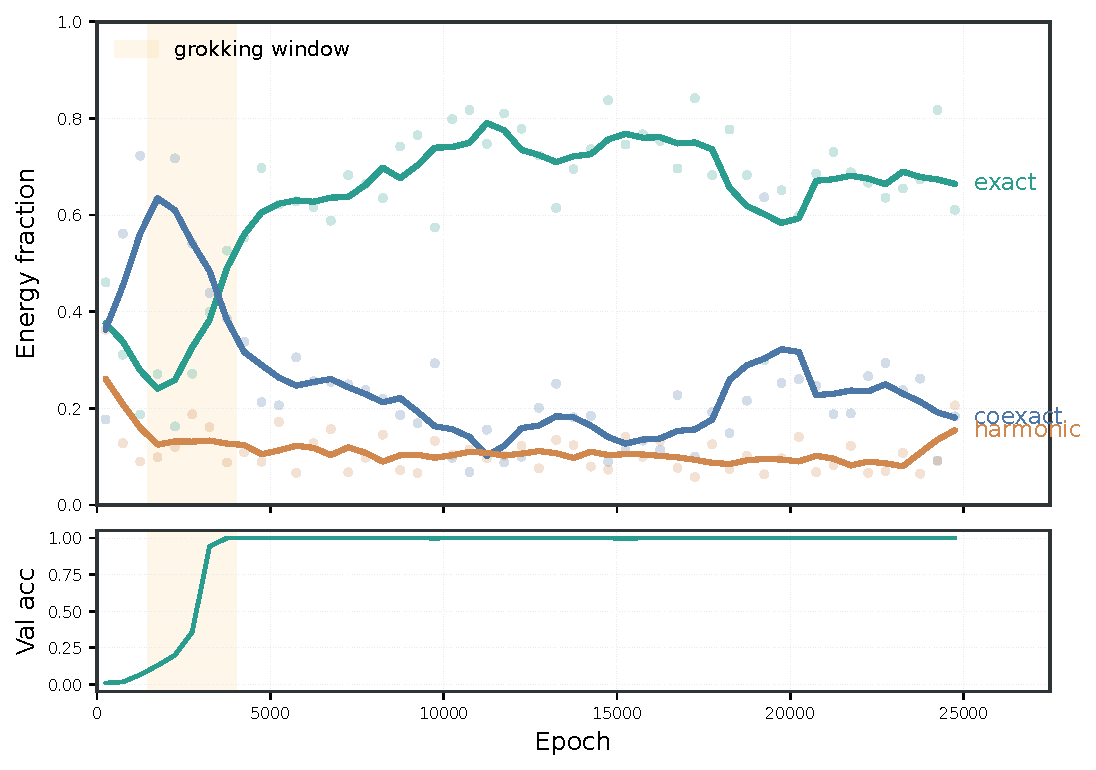
\includegraphics[width=\textwidth]{figures/fig_dg_velocity_hodge.pdf}
\caption{The displacement field changes character across grokking: early motion is curl-like, the transition is mixed, and post-grokking refinement is more gradient-like. The top panel shows exact, coexact, and harmonic energy fractions; the bottom panel shows validation accuracy.}
\label{fig:dg-velocity-hodge}
\end{figure}

\begin{figure}[htbp]
\centering
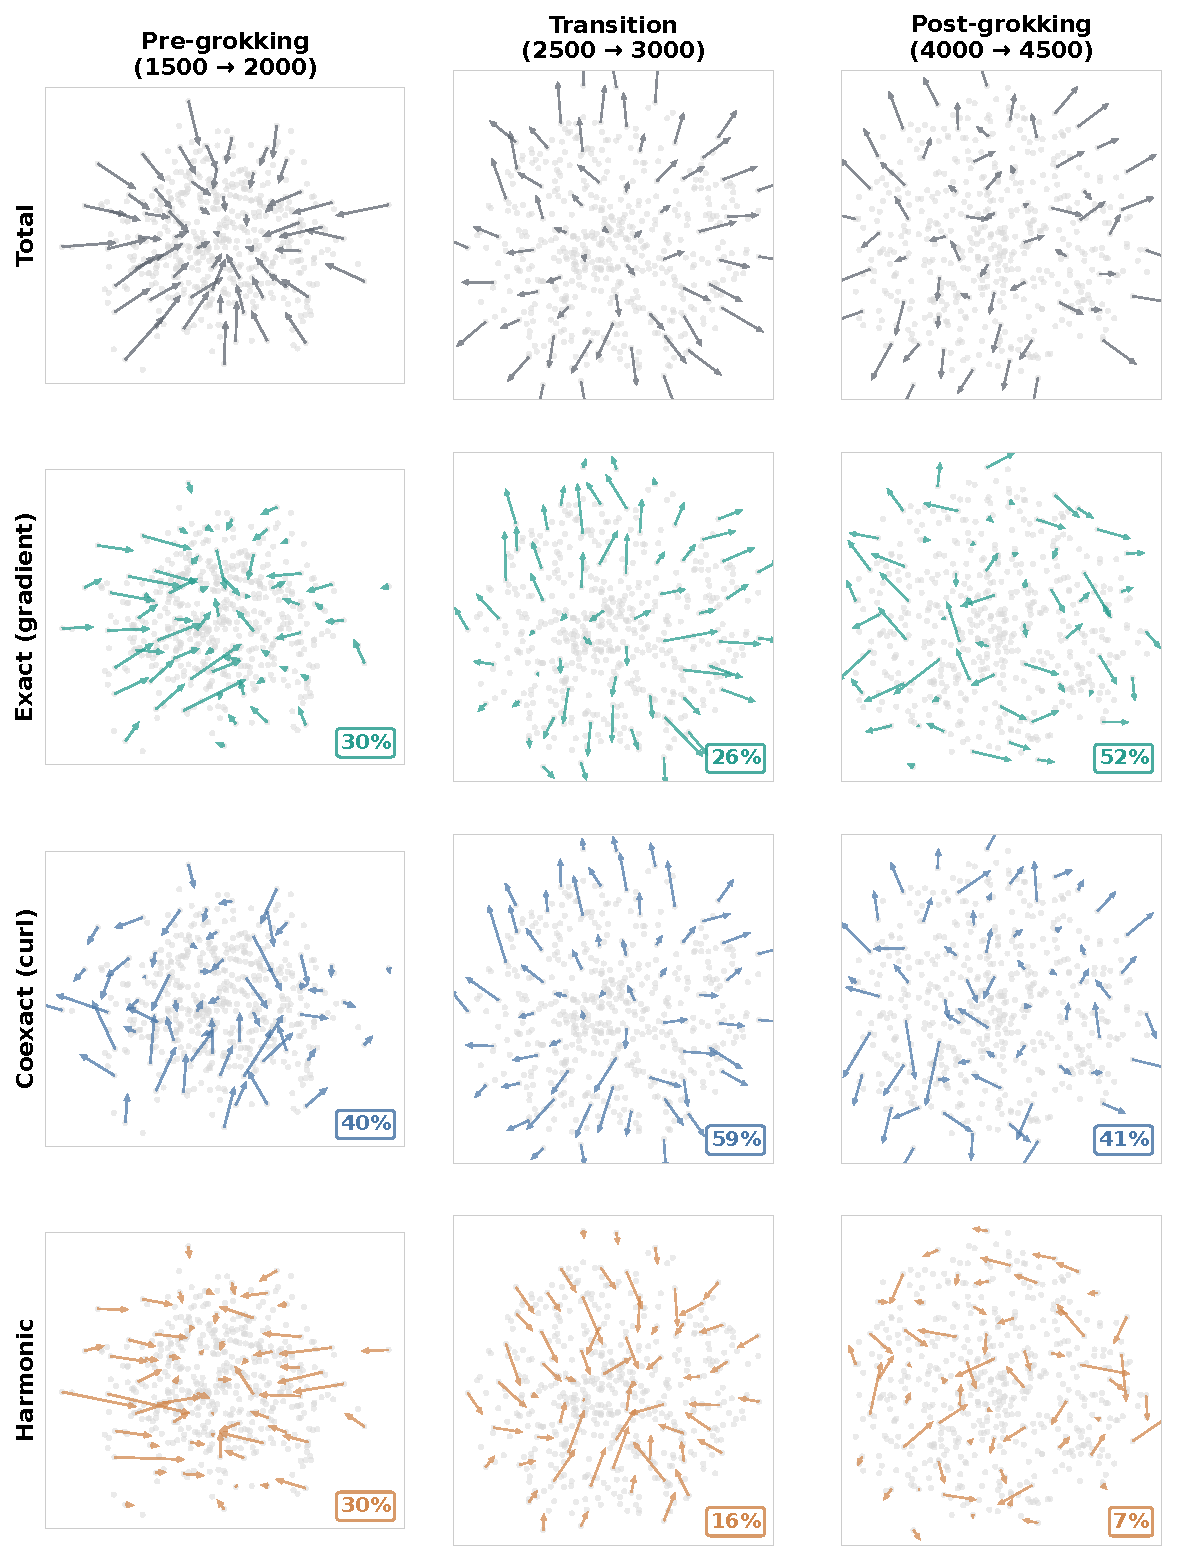
\includegraphics[width=0.85\textwidth,height=0.72\textheight,keepaspectratio]{figures/fig_dg_velocity_quiver.pdf}
\caption{Decomposed velocity fields during grokking. Columns: pre-grokking (1{,}500--2{,}000), transition (2{,}500--3{,}000), and post-grokking (4{,}000--4{,}500). Rows: total velocity, exact (gradient), coexact (curl), and harmonic. Energy fractions are annotated.}
\label{fig:dg-velocity-quiver-app}
\end{figure}

\subsection{Global Corroborating Diagnostics}

\subsubsection{Effective Dimensionality}

From the $500 \times 512$ activation matrix, prior to any PCA compression, we form the centred activation covariance $C_t$ (we do this for the same reason centering is done in PCA) and derive the effective dimension as the participation ratio
\[
d_{\mathrm{eff}}(t)
=
\frac{(\operatorname{tr} C_t)^2}{\operatorname{tr}(C_t^2)}.
\]
In other words, the ratio is the participation ratio of the covariance eigenvalues. After starting at 50.7, $d_{\mathrm{eff}}$ quickly decreases and is already down to $\sim$24 by epoch 500. It keeps dropping until reaching about 10 when grokking begins. Once past the transition, values flatten between 5 and 7, settling at $\sim 6.4$ by the final checkpoint (\Cref{fig:grokking-effdim}). What remains is supported by just a few Fourier subspaces instead of spreading across many dimensions.

\begin{figure}[htbp]
\centering
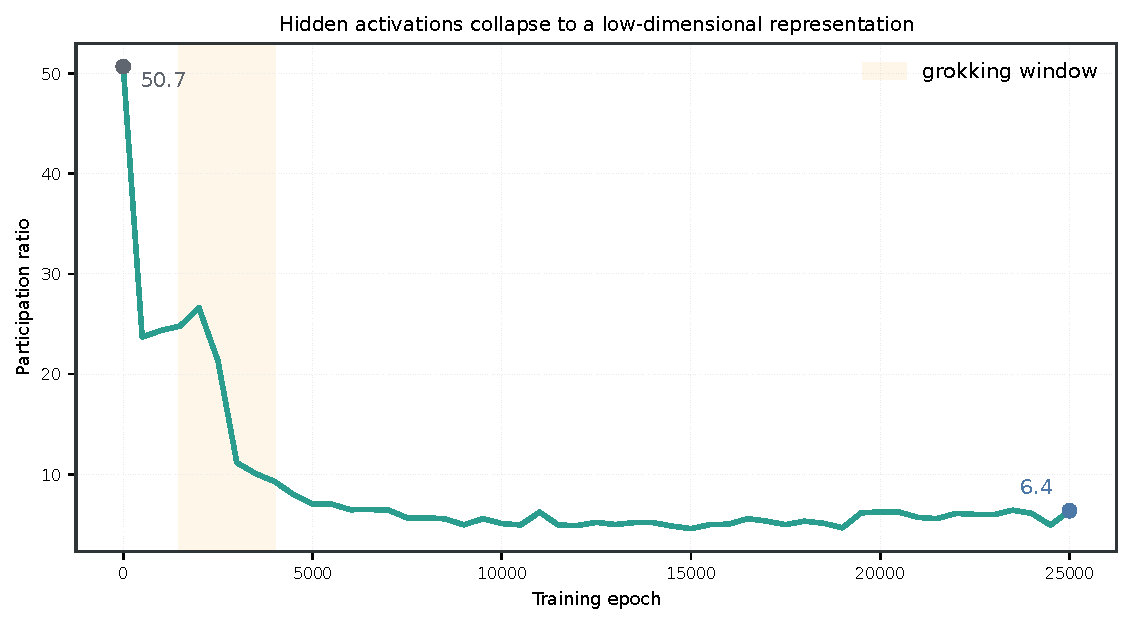
\includegraphics[width=0.9\textwidth]{figures/fig_effective_dim.pdf}
\caption{The hidden representation collapses from a diffuse high-dimensional cloud to a low-dimensional solution. The shaded window marks grokking; the curve shows the participation ratio falling from $50.7$ at initialisation to $\sim 6.4$ by the final checkpoint. The earliest compression is largest, so this figure only shows dimensional collapse in general and is not yet a complete transition marker.}
\label{fig:grokking-effdim}
\end{figure}

\subsubsection{BW Distance Between Geometric States}

The distance time series has three distinct features. The largest peak sits right at the start ($d_{\BW} = 7.34$ at epochs 0--500), as the diffuse initial geometry gives way to learned structure. A second, smaller spike appears at the grokking transition ($d_{\BW} = 1.36$ at 2{,}000--2{,}500, then $1.65$ at 2{,}500--3{,}000). After that the consecutive distance settles into a much lower band, with mean $\bar d_{\BW} \approx 0.56$ and occasional fluctuations up to $1.23$.

\section{Discussion}

This paper reveals two distinct perspectives on how geometric structure develops. First, the operator-level lens applied to $L^\dagger$. Second, the Hodge approach on the velocity field $v_i(t) = x_i(t + \Delta t) - x_i(t)$. Both sides are available because vertex identities are stable across activation clouds. The operator-side reading reflects changes in the spectrum as geometry evolves, while the movement of individual points across the manifold becomes visible through spatial analysis. As the grokking transition happens, each of these two parts shows large changes at the same time. Across successive markers, the operator distance increases steeply while the velocity field shows that the nature of the velocity Hodge decomposition changes.

\subsection{Summary of Grokking Findings}

The spatial analysis showed that, in the baseline seed, the probe velocity evolves from a coexact-dominated (curl-like, $\sim$49\%) regime during memorisation to an exact-dominated (directed, $\sim$69\%) post-grokking regime, with the exact component rising during the transition window (epochs 1{,}500 to 4{,}000). On the operator side, the BW distance between consecutive resolvent covariances has a large initial spike, a secondary increase during the grokking transition, and then a much smaller range of values post-grokking. The effective dimensionality drops from 50.7 to 6.4. After generalisation, the consecutive resolvent BW distances, velocity Hodge, and effective dimensionality converge to stable values. We interpret this to mean that the representation has reached a geometrically stable state.

\subsection{Grokking as Geometric Memory}

The grokking experiment is a concrete case study for geometric memory \citep{noroozizadeh2025geometric}. The three phases of grokking align with three modes of geometric storage.

\begin{enumerate}
    \item The first phase is pre-algorithmic memorisation (epochs 0--1{,}500). The representation forms a high-dimensional unordered arrangement that fits the training set but does not support generalisation. The BW analysis within this paper registers this as the largest geometric restructuring in the run. The effective dimensionality collapses, and the velocity Hodge decomposition shows coexact-led (curl-like) motion that increases until generalisation begins.

    \item The second phase is geometric algorithmisation (epochs 1{,}500--4{,}000). The model shifts from storing individual training examples to storing the actual \emph{algorithm} as a geometric configuration. This is the multi-frequency Fourier arrangement studied in this paper and in \citet{nanda2023progress}. It is supported by the effective dimensionality collapse and the velocity-field Hodge crossover (in the baseline seed).

    \item The third and final phase is geometric refinement (epochs 4{,}000+). The algorithmic geometry has settled, the effective dimensionality plateaus at a low value, the BW distances drop into a low band, and the velocity is exact-dominated in the baseline seed as the network fine-tunes its Fourier embedding rather than reorganising its internal representations through rotation.
\end{enumerate}

The key insight here is that memorisation and generalisation have distinct geometric signatures. The difference, therefore, is not between geometric and non-geometric storage. It is between what is stored geometrically: individual data points (memorisation) versus an algorithmic structure (generalisation). Grokking is the phase transition between these two modes of memory. The BW framework and Hodge decomposition employed in this paper delineate different aspects of the transition period, and together they illustrate algorithmic reorganisation in a neural network.

\section{Conclusion}

The primary contribution is a pointwise velocity-field Hodge decomposition across three grokking runs. The transition is clearly visible in the representation and in the operator geometry. The effective dimension of the centred activation covariance collapsed from $50.7$ to $6.4$, while the BW distance between successive resolvent operators showed a large initial spike, a smaller transition-time increase, and then stayed in a small range once the grokking period was over. The Hodge decomposition of the probe velocity field showed a crossover from coexact-guided motion to an exact-dominated field around the grokking period, but the pattern was not clear in one of the three seeds, so wider testing is needed before we can trust this crossover as a diagnostic. What we can say is that in all three seeds the transition was coexact-dominated, with coexact peaking at the start of the transition in two of them, which suggests that the representations undergo rotational shifts as they reorganise. Further, a stronger mechanistic claim would also require the Hodge decomposition to survive parameter and probe sweeps, which we were not able to complete due to resource constraints.

\appendix

\section{Supplementary Geometric Diagnostics}

\subsection{Fourier-Supervised Projection}
\label{sec:grokking-pca}

The ridge $R^2$ values reported below serve as in-sample diagnostics on a consistent set of probes. With $n < d$, the initialisation score rises artificially due to overfitting and should therefore not be read as pointing to real Fourier structure. Since the DG circular value tracks the best pair among numerous pairs of eigenfunctions, it serves better as a tool to spot top-performing pairs rather than persistent canonical coordinates.

\begin{remark}[Fourier-supervised vs unsupervised projection]
\label{rem:fourier-projection}
We found that vanilla PCA does not reliably recover the Fourier circle. Different weight initialisations orient the Fourier subspace differently inside $\mathbb{R}^{512}$ so the circle does not need to align with the leading PCs. We hence use a supervised projection via ridge regression (\Cref{sec:grokking-pca}). The ridge picks out the directions in activation space that encode a chosen Fourier frequency, regardless of how that subspace happens to sit in activation space. In the runs we checked, this projection recovers clean circles across the TransformerLens versions tested. This confirms that the Fourier structure is in the activations even when its PCA visibility depends on the seed we use.
\end{remark}

We project a $500 \times 512$ activation block into 2D by fitting ridge regressions $w_{\cos}$ and $w_{\sin}$ that predict $\cos(2\pi k \cdot \ell / P)$ and $\sin(2\pi k \cdot \ell / P)$ from activations, then scatter plot $(w_{\cos}^\top x,\ w_{\sin}^\top x)$. The plotted axes are therefore Fourier-supervised axes and not $\mathrm{PC1}, \mathrm{PC2}$. The ridge picks out the 2D affine subspace of activation space most aligned with frequency~$k$. Vanilla PCA picks the top variance subspace which, for the activations we use, does not cleanly isolate a single Fourier frequency (\Cref{rem:fourier-projection}). Finally, the ridge penalty $\alpha = 10$ matters here because the regression is in the $n < d$ regime (500 points in 512 dimensions), and the label $\ell_i = (a_i + b_i) \bmod P$ is the ground truth label.

We use the joint cos/sin $R^2$ as a diagnostic score, as it tells us how strongly the activations encode frequency. \Cref{fig:grokking-pca} displays one high-scoring Fourier mode, $k = 38$ ($R^2 = 0.994$ at the final checkpoint); other criteria, as we discuss below, pick $k = 36$ or $k = 49$ instead.

The raw PCA diagnostic and the unsupervised DG scan below identify $k_{\mathrm{dom}} = 36$ as the most stable frequency at epochs 2{,}500 and 3{,}000, with $k_{\mathrm{dom}} = 38$ at the final checkpoint. This discrepancy reflects the multi-frequency nature of the solution (a torus, not a circle). Several nearby frequencies, including $k = 36$, $38$ and $49$, all reach high post-grokking ridge scores. At initialisation the projection shows a diffuse cloud ($R^2 = 0.70$, largely reflecting in-sample overfitting in the $n < d$ regime), and by epoch 3{,}000 a clear circle has formed ($R^2 = 0.98$). Post-grokking the circle is well-defined with ordered colour strips ($R^2 \approx 0.99$).

\begin{figure}[htbp]
\centering
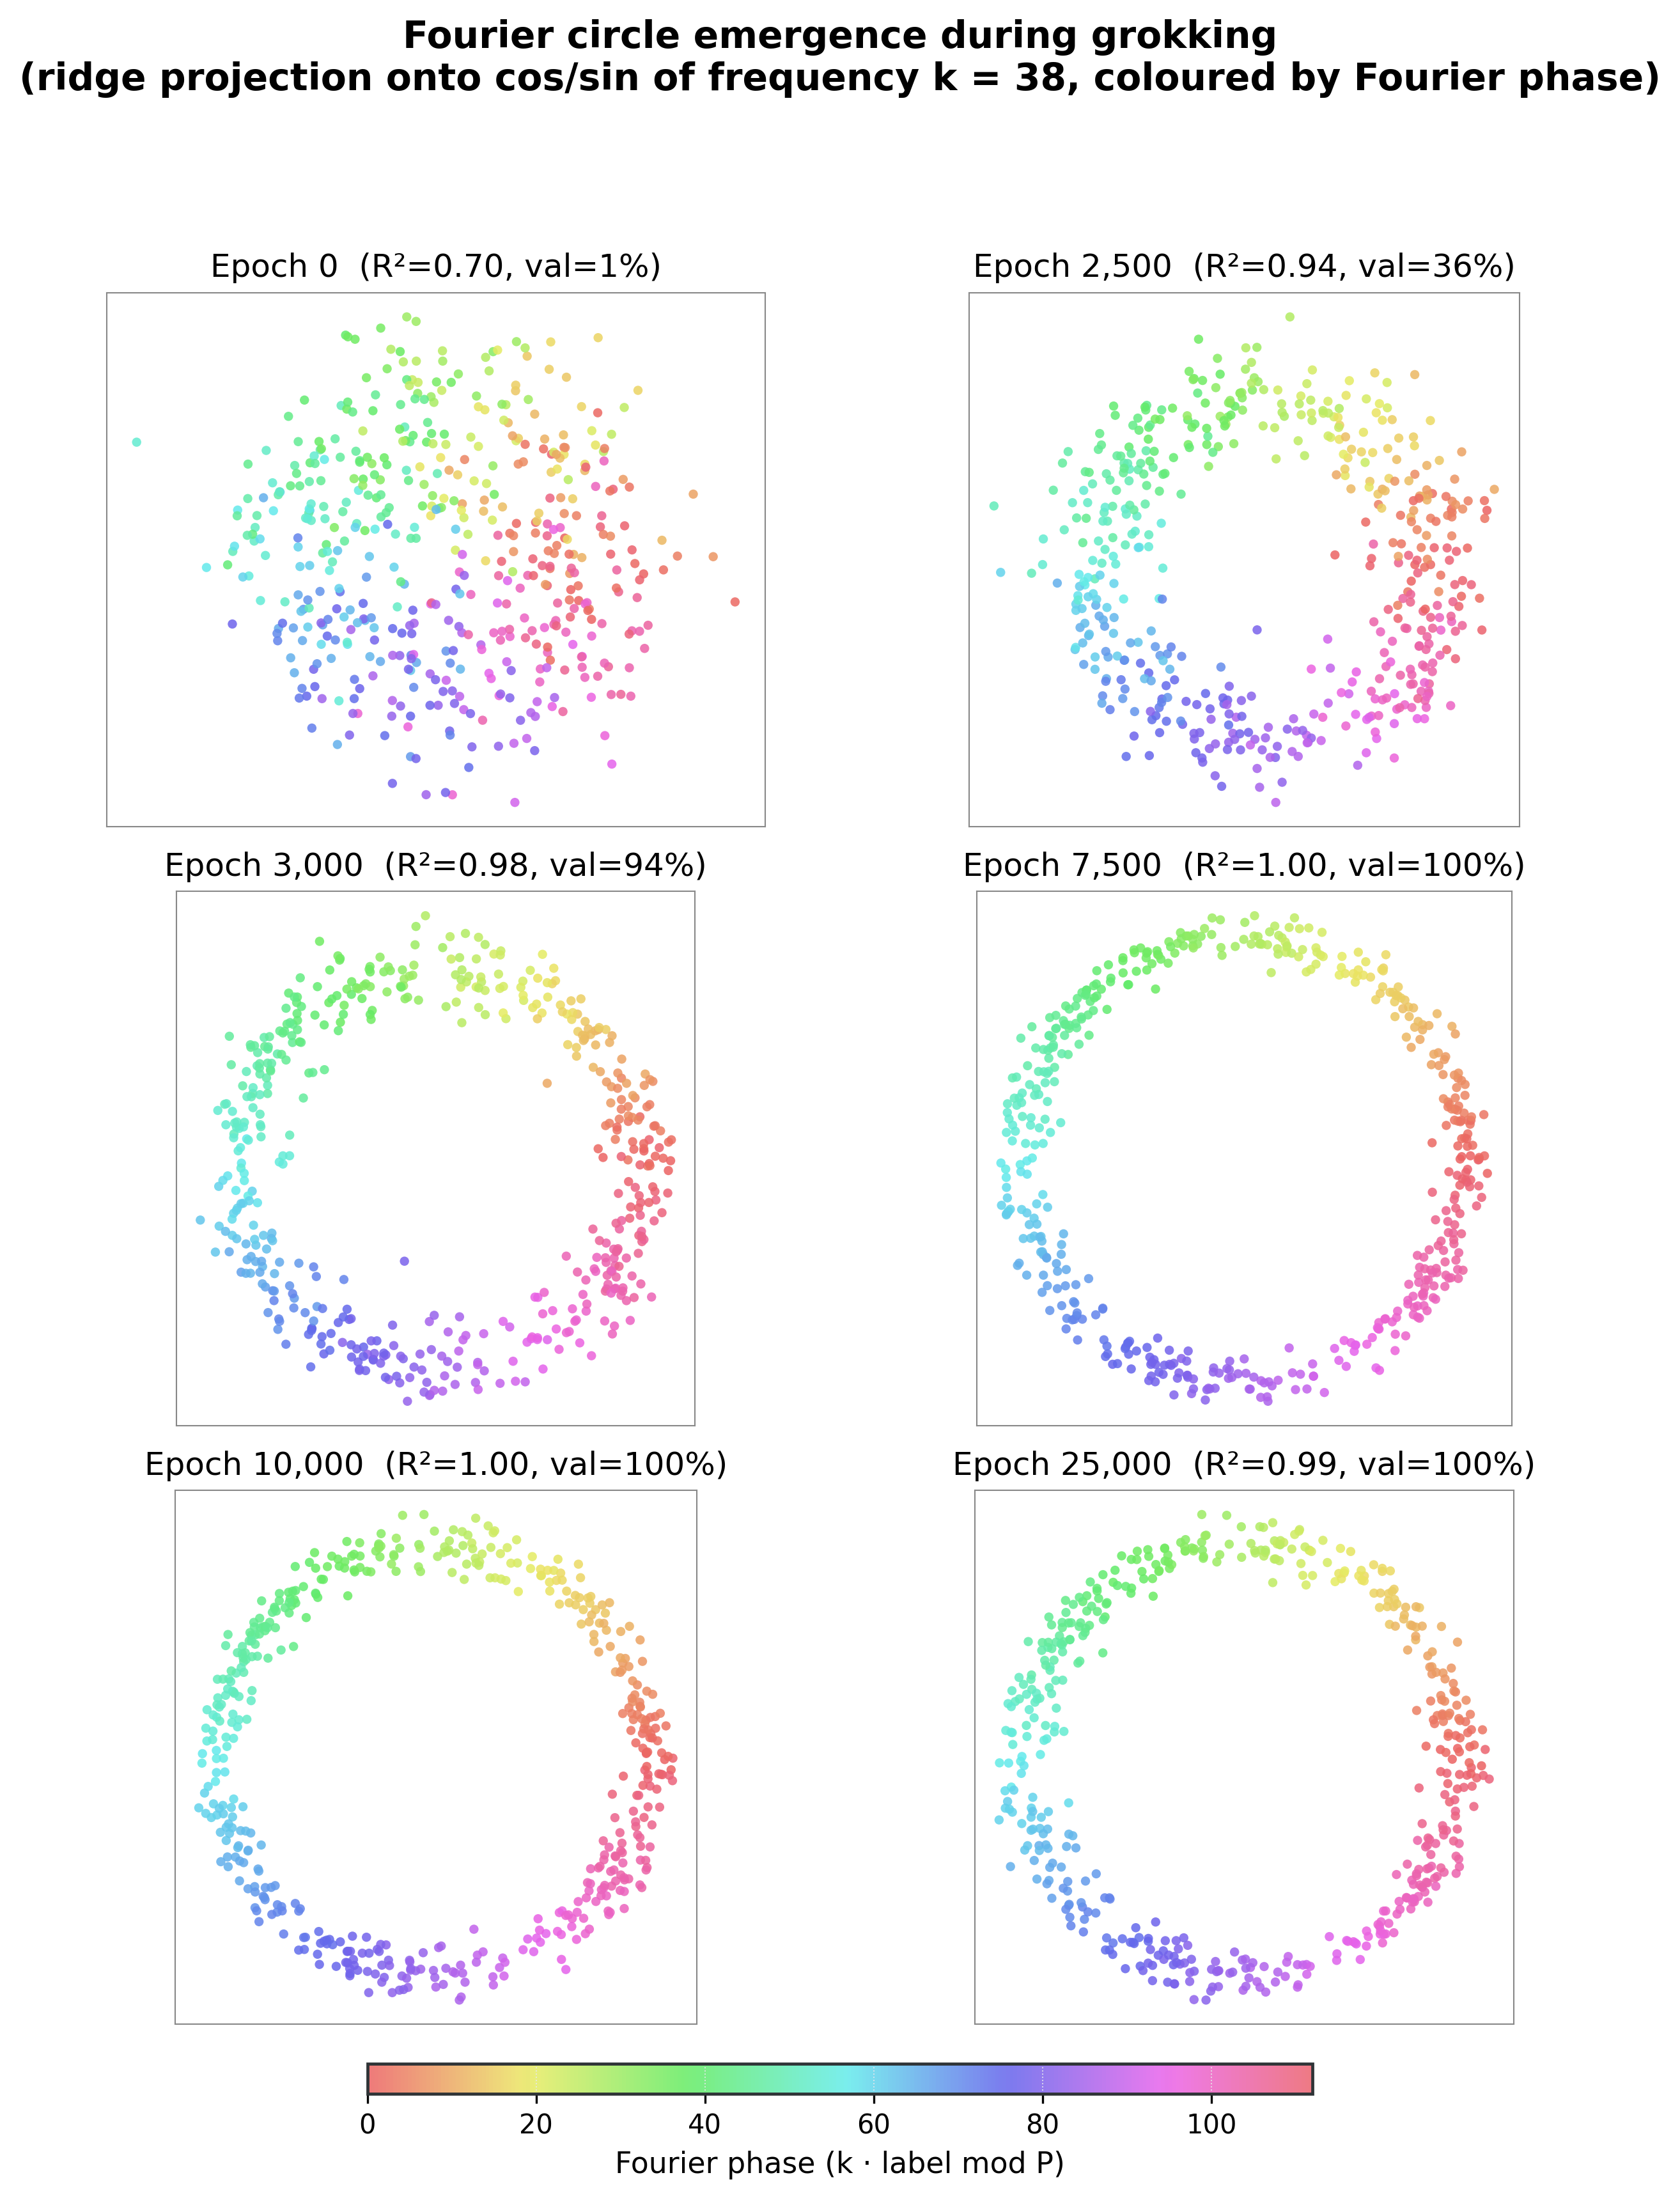
\includegraphics[width=\textwidth,height=0.72\textheight,keepaspectratio]{figures/fig_fourier_ridge_pca.png}
\caption{Fourier-supervised ridge projection of MLP hidden activations onto the strongest final-checkpoint Fourier mode, $k = 38$. Note that the plotted axes are ridge directions $(w_{\cos}^\top x,\ w_{\sin}^\top x)$ rather than principal components $(\mathrm{PC1}, \mathrm{PC2})$. Points are coloured by Fourier phase $(k \cdot \ell) \bmod P$, which aligns the colour cycle with the displayed frequency. At initialisation the projection is noisy ($R^2 = 0.70$), which reflects ridge overfitting on the probes rather than Fourier structure. By epoch 3{,}000 a clean circle emerges ($R^2 = 0.98$) with smoothly ordered colour strips, confirming that a Fourier clock solution is present in the activations.}
\label{fig:grokking-pca}
\end{figure}

\subsection{Heat Kernel Multiscale Analysis}

The complementary operator-level view replaces the resolvent covariance with the heat kernel
\[
H_t(\tau) = e^{-\tau L_t},
\]
evaluated at three scales $\tau \in \{0.1, 1.0, 10.0\}$ (local, mesoscopic, global). For consistency with the resolvent analysis, the heat-kernel BW distances are computed on the same retained non-trivial spectral subspace unless otherwise stated. The scale parameter sets the diffusion time at which the kernel is read out, so each scale exposes a different rate of geometric reorganisation.

At different scales ($\tau$ set to $0.1$, $1.0$ and $10.0$) the heat kernel delivers a clearer picture than the resolvent. While the resolvent captures broad trends, the heat kernel separates changes at distinct diffusion times. Right when training begins, the BW distance spikes at all scales and then quickly falls once that phase ends. The peak distances are 3.79 at the local scale, 3.31 at the mesoscopic scale, and 1.13 at the global scale.

Indeed the global peak is roughly one-third the local peak. Another small peak shows up across each scale near epochs 2{,}000 to 3{,}000, matching the shift into grokking. Post-grokking, the three curves settle to low baseline fluctuations.

\begin{figure}[htbp]
\centering
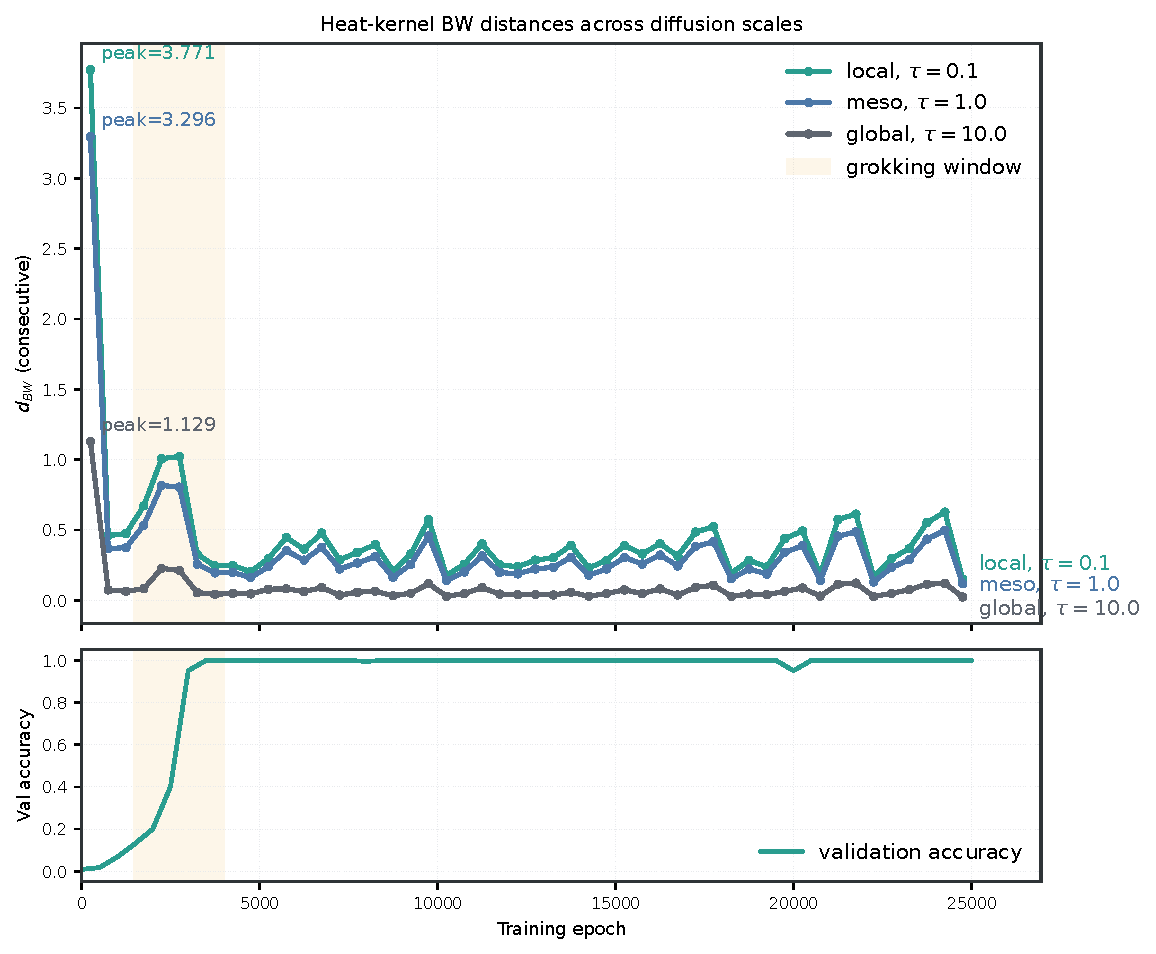
\includegraphics[width=\textwidth]{figures/fig_heat_kernel_bw.pdf}
\caption{Heat-kernel BW shows the same operator change at the grokking transition across diffusion scales with the strongest locally and the weakest globally. The curves are consecutive BW distances between heat kernels at $\tau=0.1,1.0,10.0$, with validation accuracy below. The shared shaded window makes the scale-specific increase comparable to the much larger initial restructuring.}
\label{fig:heat-kernel-bw}
\end{figure}

\section{Claims, Evidence, and Limitations}

\begin{table}[htbp]
\centering
\caption{Claims, evidence, robustness checks, and limitations for the grokking case study.}
\label{tab:grokking-claims-evidence}
\scriptsize
\setlength{\tabcolsep}{3pt}
\renewcommand{\arraystretch}{1.08}
\begin{tabular}{@{}>{\raggedright\arraybackslash}p{0.18\textwidth}%
>{\raggedright\arraybackslash}p{0.27\textwidth}%
>{\raggedright\arraybackslash}p{0.27\textwidth}%
>{\raggedright\arraybackslash}p{0.16\textwidth}@{}}
\toprule
\textbf{Claim} & \textbf{Primary evidence} & \textbf{Robustness or diagnostic check} & \textbf{Remaining limitation} \\
\midrule
Grokking has a sharp training transition &
Validation accuracy remains near chance until $\sim$1{,}500 epochs, reaches 94.3\% by 3{,}000, and reaches 100\% by 4{,}000. &
All geometric summaries are anchored to the same pre/transition/post timeline. &
Three trained seeds (598, 599, 777). \\
\addlinespace[0.2em]
Point motion changes character &
Velocity Hodge is coexact-led during memorisation and the transition window. &
Consistent with the BW/heat/operator timing and the post-grokking stabilisation. Three seeds: coexact fraction 0.49--0.58 in the transition window. &
No completed Hodge sweep. \\
\addlinespace[0.2em]
Representation dimension collapses &
Participation-ratio effective dimension falls from 50.7 at initialisation to 6.4 post-grokking. &
Four 400-example probe subsets give 49.63 $\pm$ 0.50 $\to$ 6.40 $\pm$ 0.03, ratio 0.129 $\pm$ 0.002. Three seeds give final/initial 0.126, 0.194, 0.250. &
Probe-subset and three-seed checks. \\
\addlinespace[0.2em]
Operator geometry restructures &
Resolvent BW distance has a large initial spike ($d_{\BW}=7.34$), a transition-time burst ($1.36$, $1.65$), and a lower post-grokking band. &
Probe subsets preserve the pattern: initial $6.258\pm0.050$, transition peak $1.662\pm0.057$, post mean $0.531\pm0.016$, transition/post $3.13\pm0.09$. Three seeds give transition/post 2.92, 2.64, 1.48 (2.29, 1.84, 1.44 after accuracy alignment). &
Graph, PCA, and reference-basis choices. \\
\addlinespace[0.2em]
Local diffusion geometry changes at the transition &
Heat-kernel BW curves show a secondary increase across local, meso, and global diffusion scales. &
For probe subsets, transition/post ratios are $3.12\pm0.11$ ($\tau=0.1$), $3.21\pm0.11$ ($\tau=1$), and $3.36\pm0.05$ ($\tau=10$); all four subsets have transition peak above post mean at every scale. Three seeds give $\tau=1$ peak/post 2.99, 2.47, 1.52. &
Only three diffusion scales are tested. \\
\addlinespace[0.2em]
Algorithmic Fourier structure emerges &
Fourier ridge projections and circular-coordinate scans recover post-grokking circular or multi-frequency structure. &
The result is treated as diagnostic rather than a pre-registered coordinate claim. &
In-sample ridge; best-pair circular scan; correlation varies in seeds 599 and 777. \\
\bottomrule
\end{tabular}
\renewcommand{\arraystretch}{1.0}
\end{table}

\Cref{tab:grokking-claims-evidence} also identifies what would weaken our interpretation. The analysis on the operator side held under three independent training seeds for the dimensionality collapse and the BW spikes during the grokking transition. However, it could still lose its persuasiveness if those effects disappeared under held-out probe resampling. Further, a stronger mechanistic claim would also require the Hodge decomposition and circular coordinate diagnostics to survive parameter and probe sweeps, which we were not able to complete due to resource constraints.

\bibliographystyle{plainnat}
\bibliography{references}

\end{document}
